%% Intended to be included into a larger document
\chapter{Related Works}

%% Add more to introduce topics in this chapter?

\section{Why Games}
\label{sec:why-games}

Gamification is not about games, in fact as a subject gamification is deals with everything else but games. But the research in gamification have to largely base on the studies of games. The games already prove to be an effective engaging media and ubiquitous as every day life. In fact, "video game is everywhere" is the critical thesis of many gamification advocates. 

[need more data on game market, player demography]

The following sections will examine a few most popular games and genre to understand what game mechanics give games such power nowaday.

\subsection{Casual Game: Angry Birds}
In today's tech world, no gaming platform is completed without the new star game Angry Birds. There  are over 50 million individuals have downloaded this simple game. The total number of hours consumed by world-wide players is roughly 200 million minutes a day, that is 1.2 billion hours a year.  According to Neiman Journalism Lab[ref], all person-hours spent creating and updating the entire wikipedia totals about 100 million hours.  That is half day of the Angry Birds play time. Why is this seemly simple game so massively compelling? Charles Mauro [ref] discussed the cognitive teardown of Angry Birds in Human factor engineering (aka usability engineering) for the sake of answering the more "important" real world question, "why users don't find their company's software or product engaging?":

    * Simple Engaging Interaction Concept:
    Angry Birds' simple interaction model is easy to learn and incremental increase of complexity.

    * Cleverly managed response time: 
    In Angry Birds design, it is not "faster is better", instead, different birds have different trajectory time and the flight path of the bird is intentionally illustrated. It solved one huge problem for user interfaces - error correction.It also take a seemly long time for the pigs to expire once their hours are collapsed, this non-functional time delay increases the playfulness of the game and bring users entertainment.

\subsection{Social Game: Zynga-Ville}
With the motto  "Connecting the world through games", Zynga who found in 2007 quickly become the top game company catching up to the more traditional establishment such as EA and Activision Blizzard. With the help of socal network platform Facebook, the FarmVille and CityVille quickly become the most popular games within Facebook. Zynga later expanded the games into other platform such as mobile and  new google+ social network. 

[more research on Zynga's game number, total time played, total player, compared to Angry Birds]

One distinct characteristic of Zynga games is that they are social and they are all interconnect through an exchangable virtual currency "Zynga Points". 

[more on virtual currency's social effect]

\subsection{MMORPG: World of Warcraft}

\section{Game Theory}

\subsection{Flow}
Psychology professor Mihaly Czikszentmihalyi introduced a specific kind of happiness that he named "flow", which is widely accepted to be one of the fundamental reasons that people play games. Flow, a state of absorption in one's work, is characterized by intense concentration, loss of self-awareness, a feeling of being perfrectly challenged (neither bored nor overwhelmed) and a sense that time if flying. 

As Csikszentmihalyi describes (Csikszentmihalyi 1990), there are seven core components of flow that are summarized in Table 2.1. These components can be broken into two categories: conditions and characteristics. Conditions must be achieved before flow can be reached. Characteristics occur while a person is in flow, even though they may be unaware of it.

\begin{table}[ht]
  \centering
    \caption{Flow Condition and Characteristics}
    \begin{tabular}{ | l | p {10cm} |}
    \hline
    Conditions of Flow & Explanation \\ \hline
    Clear tasks & Person understands what they must complete  \\ \hline
    Feedback & Person receives clear and immediate feedback showing what succeeds and what fails \\ \hline
    Concentration/focus & Person is not distracted and can fully attend to the task \\ \hline
    An attainable, balanced goal & Goal is challenging and within their abilities to complete \\ \hline
    Characteristics of Flow & Explanation \\ \hline
    Control & Person believes their actions have direct impact on tasks and that they can control the outcome \\   \hline
    Diminished awareness of self & Complete focus on the task leaves little room for feeling self-conscious or doubt. Often described as becoming a part of the activity. \\ \hline
    Altered sense of time & Perception of time is distorted. Seconds can feel like minutes, minutes like hours. Yet, time also passes by quickly, unnoticed. \\ \hline
    \end{tabular}
\end{table}

In order to achieve the flow, the right conditions above must exist. The last and the most important condition is a balanced goal that is challenging yet achievable within the individaul's ability. A task that is not challenging or  requires excessive time to complete becomes boring and players lose interest; A task that is too hard causes frustration and anxiety and again players lose interest. With a person’s skills improve over time, the challenge needs to increase along with the improving skills. This balance is referred to as the flow channel as shown in figure 2.1 (based on a diagram from Csikszentmihalyi, 1990, p 74).

\begin{figure}[ht]
	\centering
		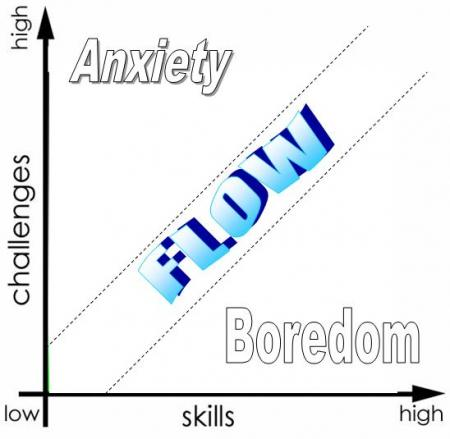
\includegraphics[scale=0.59]{czikszentmihalyi.jpg}
		\caption{The state of flow is achieved between anxiety and boredom}
		\label{fig:state_of_flow}
\end{figure}

\subsection{Player Type}
In order to understand why people play games, Ricahrd Bartle identified four player personality types by studying players of MMOGs (massively multiplayer online games), as shown in Figure 2.2

\begin{figure}[ht]
	\centering
		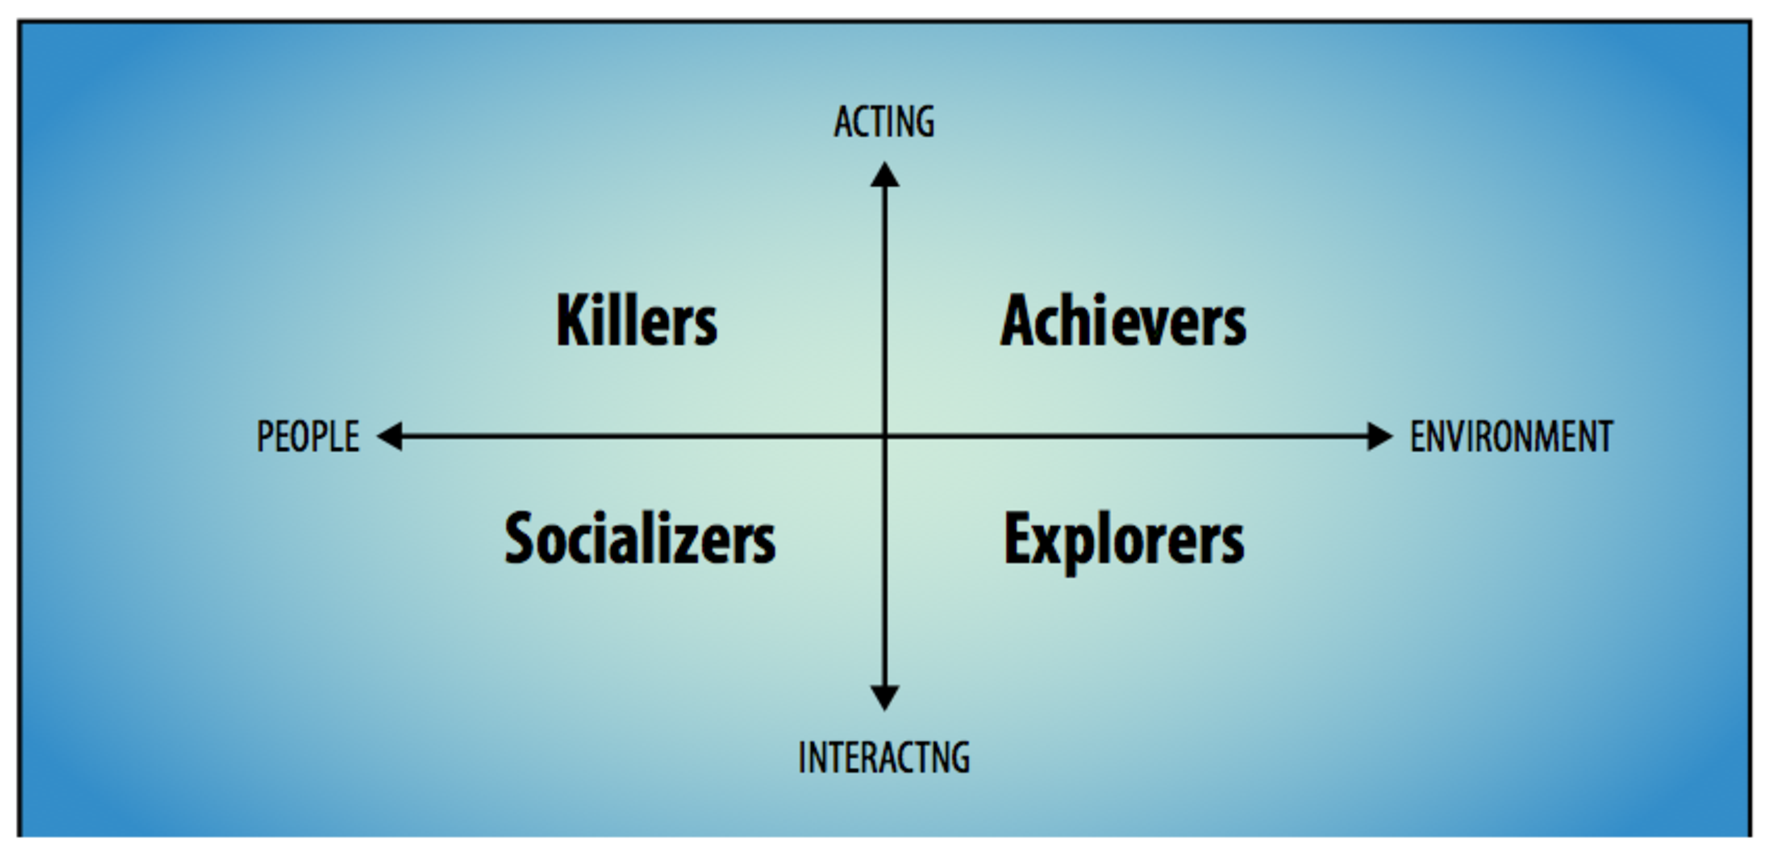
\includegraphics[scale=0.59]{bartle_player_type.pdf}
		\caption{Bartle's Player Types}
		\label{fig:player_types}
\end{figure}

1. Explorers have a clear inclination towards discovery

2. Achievers are definitely motivated by the accumulation of experience points, status and ranks associated with their proficient use of the software

3. Killers are motivated by challenge, competition, and the rapid pace of usage as in a first-person shooter game.

4. Socializers like to socialize in a collaborative non-confrontational environment.
 
One study [ref?] found that approximately 80\% of the populations are Socializers. Explorers, achievers and killers make up only about 20\% of the population.

\subsection{Fogg Behavior Model}
Stanford University's researcher BJ Fogg [ref] introduces the Fogg Behavior Model (FBM) to explain what causes behavior change. The model shows that three elements, Motivation, Ability, and Trigger must converge at the same moment for a behavior to occur. 

\begin{figure}[ht]
	\centering
		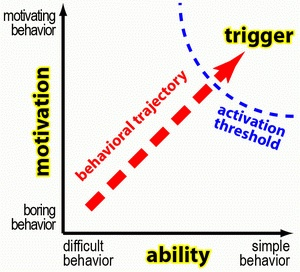
\includegraphics[scale=0.59]{fogg_behavior_model.jpg}
		\caption{Fogg Behavior Model}
		\label{fig:behavior_model}
\end{figure}

1. Motivation: the person wants desperately to perform the behavior (i.e. he is highly motivated)

2.Ability: the person can easily carry out the behavior (i.e. he considers the behavior very simple)

3. Trigger: the person is triggered to do the behavior (i.e. he is cued, reminded, asked, called to action, etc.)
 
Michael Wu [ref] uses FBM to analyze why and how gamification are able to drive actions. 
"Game mechanics and game dynamics are able to positively influence human behavior because they are designed to drive the players above the activation threshold (i.e. the upper right of the ability-motivation axis), and then trigger them into specific actions. In other words, successful gamification is all about making these three factors occur at the same time."

\section{Game Mechanics}
There are many game mechanics make game a game. 

\subsection{Status}
This include experience points(XP), ranks on the leader board, health.

\subsection{Achievement}
This normally represents as badge, completed quests.

\subsection{Level progression}

\subsection{Mission Quest Journey}

\subsection{Social}

\subsection{Virtual good or Real-world tangibles reward}

\subsection{Immediate feedback}

\section{Gamification Debates}
"As game techniques infiltrate walks of life outside of the traditional online gaming universe, however, some are condemning its application in these new spheres. At the Wharton conference, Georgia Institute of Technology professor and game designer Ian Bogost called gamification efforts "exploitation-ware" that is being "invented by consultants as a means to capture the wild, coveted beast that is video games and to domesticate it for use in the grey, hopeless wasteland of big business." Gamification, he argued, "gets games wrong, mistaking incidental properties like points and levels for primary features like interactions with behavioral complexity."

But Gabe Zichermann, an author, entrepreneur and blogger at the online industry community Gamification Co., countered that gamification is not only a new industry that can create thousands of jobs for game designers and others, but is also a field that will yield benefits for the public. "It's the meaning we will enrich, educations we will improve, health we will foster and lives we will lengthen through the application of gamification design that will be among our most important legacies," he noted.

As an example, Zichermann cited non-profit HopeLab's use of game techniques to fight obesity among low-income teens. Equipped with an accelerometer measuring vigorous activity, teens can boost their online status through exercise and gain "Zamz," a virtual currency that can be used to purchase online and real-world rewards. HopeLab reported that participating teens' activity levels increased by 30% a month through this process.

To Trick or Transform?

Still, debate continues over whether gamification itself is inherently good or bad. That is, is its use motivated by bad intentions to dupe people into doing things that aren't necessarily in their best interest? Or are some attempts at gamification merely poorly executed, so that its effects are superficial and fail to transform people's behavior in long-lasting, positive ways? "If gamification is fundamentally about tricking people to feel happier about situations that aren't going to be better [for them], then it's problematic on a lot of levels -- both ethically and in effectiveness in the long term," according to Kevin Werbach, a Wharton professor of legal studies and business ethics who organized the conference with Dan Hunter, a professor at New York Law School. "The question is: What are the aspects of [gamification] that are really about meaningfully improving people's experience?"

Gamification is naturally suspect if it is used by corporations, terrorist organizations or others with the intention of potentially causing harm -- whether to push the sales of useless products and services like subprime mortgages, or to lure recruits into suicide missions. Even if the goals of gamification are exemplary, however, does gamification merely gloss over real problems that require real answers? For example, does awarding participants points and using other incentives through the HopeLab program significantly impact the root causes of teen obesity in low-income neighborhoods, such as the lack of access to, and the high price of, fresh fruits and vegetables? By gamifying the problem, "you're spreading butter over toast so it tastes better, but it doesn't solve the problem," Georgia Tech's Bogost pointed out.

Current efforts at gamification come with other pros and cons, including the relative value of extrinsic motivators (such as points, badges and rewards) versus intrinsic motivators generated by an individual's internal will or desires. "In the long run, [extrinsic rewards] are not fun," said Nicole Lazzaro, Founder of XEODesign, which helps companies such as Sony, Sega and Leapfrog improve player experiences. "The use of extrinsic motivation will decrease motivation to use your products and services once you remove that reward.... You have to keep upping the dose to have the same motivation and change in behavior over time."

But Carnegie Mellon's Schell cautioned against writing off extrinsic rewards without a deeper understanding of the psychology behind motivation. "We don't fully grasp the complex relationship between intrinsic and extrinsic rewards," he noted. And extrinsic rewards can be a catalyst for intrinsic motivation, added Michael Wu, chief scientist of Lithium Technologies, a social networking research and consulting firm. "Using an extrinsic reward is a good way to get people to start doing something," he said. Although the outside incentive may be the initial reason that people adopted a particular activity, Wu suggested that they may ultimately develop internal motivators. Once teens start losing weight and looking better, spurred by the lure of HopeLab's Zamz currency, for example, they may embrace a healthier lifestyle because it makes them feel better about themselves.

Conference panelists Sebastian Deterding of the Hans Bredow Institute in Germany and Scott Rigby, president of customer engagement research consortium Immersyve, have studied the psychology of motivation that makes online games so engaging. Online games are voluntary experiences that become so addictive that "people [who play them] won't even go to the bathroom [in the middle of a game]," Rigby pointed out. An adherent of self-determination theory, Rigby said that humans, who are "energized to grow and to elaborate ourselves," have basic psychological needs for mastery, connectedness and autonomy. If online games satisfy these basic needs, they will be highly motivating -- no matter whether the reward mechanism is extrinsic or intrinsic. In a similar vein, Deterding noted that people play games because it's "fun," which can be distilled to the freedom an individual enjoys in various forms of voluntary play.

In a field rife with anecdotes but little hard data, Wharton's Werbach and New York Law School's Hunter intend to develop in-depth case studies to examine the types of business problems organizations want gamification to solve, the techniques used and the results. According to Werbach, there currently are few bridges between game design as a craft and psychological research. "That's why research is valuable -- to get beyond whether gamification is good or bad, and does it work or not."

"

\subsection{Can you gamify a suicide hotline?}
Can you gamify everything? "No, you can not gamify game". According to Gabe Zichermann, the idea of baking game mechanics into everything you do is fun, but when asked how would you make a suicide hotline fun, he admitted that adding games to a suicide prevention seems distasteful at first, but he could add a game mechanics like a competitive environment in a call center setting.

\subsection{Gamification is bull*it}

\subsection{Gamification vs Serious game}
Serious game are generally defined[ref], �to include games that make use of computer technology and advanced video graphics and that are used for the purposes of learning and training.�

\section{How to use game mechanics in gamification}

\subsection{Gamification Applications}

\subsection{Smart Gamification}
"Carnegie Mellon University professor and game designer Jesse Schell, who ignited much of the current interest in gamification with a keynote address at the 2010 Design Innovate Communicate Entertain (D.I.C.E.) Summit, said he was surprised people took interest in his presentation, since he had talked about the phenomenon for years with little response. "Something in the air crystallized at that time," he noted. "There is something that's happening in culture right now -- a shift just as sure as the Industrial Revolution was a shift. We're moving from a time when life was all about survival to a time when it was about efficiency into a new era where design is largely about what's pleasurable." According to Schell, gamification is a way to arrive at a "fundamental understanding of what it is that's pleasurable to people." What's more, online games have entered the mainstream, helped by platforms such as smartphones, tablets and Facebook."

\section{Gamification Service or Platform}
This section outlines the current industry players that provides gamifcation service via platforms or consultation service. [see figure 2.1]

\begin{figure}[ht]
	\centering
		
\includegraphics[scale=0.59]{gamification-service.pdf}
		\caption{Gamification Service Industry}
		\label{fig:gamification-service}
\end{figure}


\subsection{Gamification Analytics}
The objective evaluation of Player Experience (PX)[ref] in games is the goal of game metrics and analytics research. With the technology advancement, it is possible to automatically log numerical informations on in-game player behaviour and analyze them in different context. This methodology provides a qualitative and quantitative result of the player experience in games, which in turn affect the result of gamification.



